% =====================================================================
%  Chapter 23 — Harvesting
% =====================================================================

\chapter{Harvesting: The Physics and the Arithmetic}
\label{ch:harvest}

The most literal reading of ``have we already tapped it'' is the one that
gets the least attention, because it sounds like science fiction and because
the honest answer requires a number ten orders of magnitude away from
anything useful. It is worth doing carefully, because the arithmetic is
instructive and because a reader who has heard the claim made badly should
be able to see exactly where it goes wrong.

\section{The proposal}The proposal, in its clearest form, is this. The Solar
System is moving through the galactic dark matter halo at about
300~km\,s$^{-1}$. Some fraction of the halo particles is gravitationally
captured by the Sun and the planets. A captured particle eventually
annihilates with another captured particle, and the annihilation products
carry away energy that was previously locked in the captured population. If
the capture and annihilation proceed, the Solar System is a dark matter
engine.

Sikivie's 2015 paper computed the resulting energy release and obtained a
figure of order $10^{35}$~TW\,yr per cubic parsec of the captured
population \idx{Sikivie}. That is the number that circulates.

\begin{figure}[!htbp]
\centering
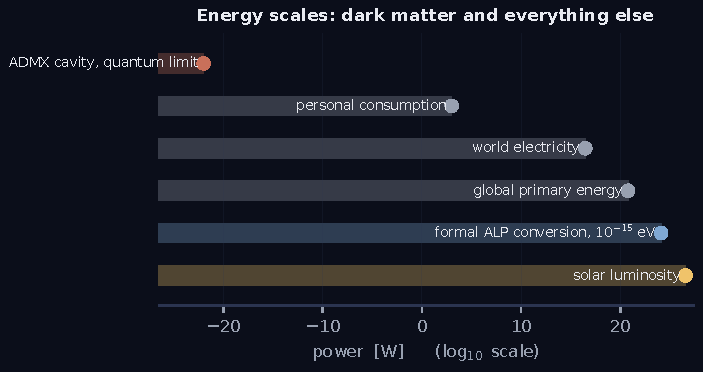
\includegraphics[width=\textwidth]{../figures/fig_energy.pdf}
\caption{The energy scales, on a logarithmic power axis. The marker on each
row is the value; the bar is drawn from the left of the scale so that the
magnitudes are comparable. The gap between the best conversion limit
available for a candidate and the Sun's output is the story of this
chapter.}
\label{fig:energy}
\end{figure}

\section{The units}The figure deserves to be read carefully, because it is
larger than anything else in the discussion.

\begin{table}[H]
\centering
\caption{Energy scales for comparison. The power figures are given in
terawatts where possible; the last row is an energy rate per unit volume
and is not directly comparable with the rows above it.}
\label{tab:energy}
\begin{tabular}{@{}>{\RaggedRight\arraybackslash}p{0.52\textwidth}l@{}}
\toprule
\textbf{Quantity} & \textbf{Value} \\
\midrule
Personal power consumption & $\sim 10^{3}$~W \\
World electricity production & $\sim 3\times 10^{4}$~TW \\
Global primary energy use & $\sim 6\times 10^{8}$~TW \\
Solar luminosity & $\sim 3.8\times 10^{14}$~TW \\
Formal ALP conversion at $10^{-15}$~eV & $\sim 1.3\times 10^{12}$~TW \\
ADMX cavity power at the quantum limit & $\sim 10^{-22}$~W \\
\bottomrule
\end{tabular}
\end{table}

The solar luminosity is $3.8\times 10^{26}$~W, so the formal ALP figure is
about one three-hundredth of the Sun's output. Against world electricity it
is about forty million times larger. These are not small numbers.

The Sikivie figure, $10^{35}$~TW\,yr per cubic parsec, is roughly
$10^{13}$ times the Sun's entire annual output, and it is a rate per unit
volume rather than an absolute rate. The numbers are large enough that the
proposal is not absurd on energy grounds.

\section{Why the numbers do not translate into power}Three separate factors
break the connection between the formal figures and anything realisable, and
it is worth separating them, because they are usually conflated.

The first is the \emph{available mass}. The captured population is a tiny
fraction of the halo population passing through the Solar System, and the
harvest rate is limited by the capture rate. Sikivie's figure is an upper
bound assuming the entire captured population is available for
annihilation.

The second is the \emph{annihilation rate}. The captured population is cold:
its velocities are tens of kilometres per second, a factor of ten below the
halo. For any candidate whose annihilation cross section is velocity-
suppressed --- and for a thermal relic the standard $s$-wave and
$p$-wave cases are --- the annihilation rate at those velocities is
suppressed by the same velocity factors. The cold captured population is
the worst possible fuel for a reaction whose rate depends on the
participants meeting each other.

The third is the \emph{coupling}. For the axion, the conversion to
electromagnetic energy happens at a rate set by $g_{a\gamma\gamma}$, and the
power available in a resonant cavity at the quantum limit is of order
$10^{-22}$~W. That is a number to sit with: the resonant conversion limit
for one of the best-understood candidates in the field is forty-eight orders
of magnitude below the Sun's output.

\section{The formal figures, read correctly}The formal ALP power figure of
$10^{12}$~TW assumes a coupling that is optimistic by roughly the factor
that the experiments exclude, and it assumes the whole local field can be
converted, which requires a device that has no existence. The correct
reading of these numbers is not that dark matter is a vast energy source.
It is that the energy content of the local dark matter is enormous compared
with human energy use --- which is true, and is a statement about how small
our energy budget is --- while the interaction that would let us reach it is
absent by ten orders of magnitude.

The energy density of dark matter in the Solar System's inner region is
roughly $10^{-2}$~J/m\(^{3}\), comparable to a terrestrial laboratory
vacuum and many orders of magnitude above the energy density of
civilisation. The dark matter is everywhere, in enormous quantity. It is
also, as far as anyone knows, completely inaccessible.

\section{What this sense is worth}It is worth two things.

The first is that it defines the target. A power technology based on dark
matter requires a coupling some ten orders of magnitude larger than anything
in nature, or a completely different production scenario in which the dark
matter is not cold and not weakly coupled. Both possibilities are excluded by
existing physics. That is a clean, decidable statement.

The second is that it disciplines the rhetoric. The dark matter is not
``free energy''. It is a locked resource with a key that does not exist in
nature. Any account that implies otherwise is making an arithmetic error,
and the field's exposure to that error grows as the resource's abundance is
quoted more often and its accessibility less.

\begin{keytakeaways}
\item The energy content of the local dark matter is enormous compared with
human energy use, and the formal conversion figures are correspondingly
large.
\item Three factors break the connection to reality: the tiny available mass,
the velocity suppression of annihilation in the cold captured population,
and the size of the coupling.
\item The resonant conversion limit for the axion is of order
$10^{-22}$~W --- forty-eight orders of magnitude below the Sun's output.
\item The honest conclusion is that the coupling does not exist in nature, and
that this is a decidable statement rather than an open question.
\end{keytakeaways}
